

\documentclass[a4paper,12pt]{article} % тип документа

% report, book

% Рисунки
\usepackage{graphicx}
\usepackage{wrapfig}

\usepackage{hyperref}
\usepackage[rgb]{xcolor}
\hypersetup{				% Гиперссылки
    colorlinks=true,       	% false: ссылки в рамках
	urlcolor=blue          % на URL
}

%  Русский язык

\usepackage[T2A]{fontenc}			% кодировка
\usepackage[utf8]{inputenc}			% кодировка исходного текста
\usepackage[english,russian]{babel}	% локализация и переносы


% Математика
\usepackage{amsmath,amsfonts,amssymb,amsthm,mathtools} 


\usepackage{wasysym}

\author{Анна Назарчук Б02-109}
\title{1.1.4 Измерение интенсивности радиационного фона}
\date{}
\begin{document}
\maketitle

\section{Аннотация}
В работе измеряется интенсивность радиационного фона, большую часть которого составляет поток космических частиц. Он изменяется со временем случайным образом и фиксируется при помощи счетчика Гейгера-Мюллера (СТС-6). Применяются методы обработки экспериментальных данных для изучение статистических закономерностей при измерении интенсивности радиационного фона.

\section{Теоретические сведения}
Регистрация частиц однородна по времени и каждое последующее событие не зависит от предыдущего, поэтому количество отсчетов в одном опыте подчиняются распределнию Пуассона, которое при больших ислах стремится к нормальному. Стандартная ошибка отдельного измерения через измеренное значение $n$:
\begin{equation}\label{сигма}
\sigma=\sqrt{n}
\end{equation}
Отсюда следует, что результат измерений с высокой точностью записывается так: 
\begin{equation}\label{н0}
n_0=n\pm\sqrt{n}
\end{equation}
При $N$ измерениях среднее значение числа частиц за одно измерений равно:
\begin{equation}\label{нср}
\overline{n}=\frac{1}{N}\sum_{i=1}^{N} {n_i}
\end{equation} 
Стандартную ошибку измерения можно оценить по формуле: 
\begin{equation}\label{сигмаотд}
\sigma_{\text{отд}}=\sqrt{\frac{1}{N}\sum_{i=1}^{N}{(n_i-\overline{n})^2}}
\end{equation}
Ближе всего к значению $ \sigma_{\text{отд}} $ лежит величина $ \sqrt{\overline{n}} $, то есть:
\begin{equation}
\label{сигмаотдприб}
\sigma_{\text{отд}}\thickapprox\sqrt{{\overline{n}}}
\end{equation}
Величина $\overline{n}$ не вполне точно совпадает с истинным значением $n_0$ и является случайной величиной. Стандартная ошибка отклонения $\overline{n}$ от $n_0$ может быть определена так:
\begin{equation}\label{сигманср}
\sigma_{\overline{n}}=\frac{1}{N}\sqrt{\sum_{i=1}^N{(n_i-\overline{n})^2}}=\frac{\sigma_{\text{отд}}}{\sqrt{N}}
\end{equation}
Относительная ошибка отдельного измерения (ожидаемое отличие любого из $n_i$ от $n_0$):
\begin{equation}
\varepsilon_{\text{отд}}=\frac{\sigma_{\text{отд}}}{n_i}\thickapprox\frac{1}{\sqrt{n_i}}
\end{equation}
Аналогично определяется относительная ошибка в определении среднего по всем измерениям значения $\overline{n}$:
\begin{equation}
\varepsilon_{\overline{n}}=\frac{\sigma_{\overline{n}}}{\overline{n}}=\frac{\sigma_{\text{отд}}}{\overline{n}\sqrt{N}}\thickapprox\frac{1}{\sqrt{\overline{n}N}}
\end{equation}
\section{Оборудование}

\begin{wrapfigure}{R}{0.2\textwidth}
\centering
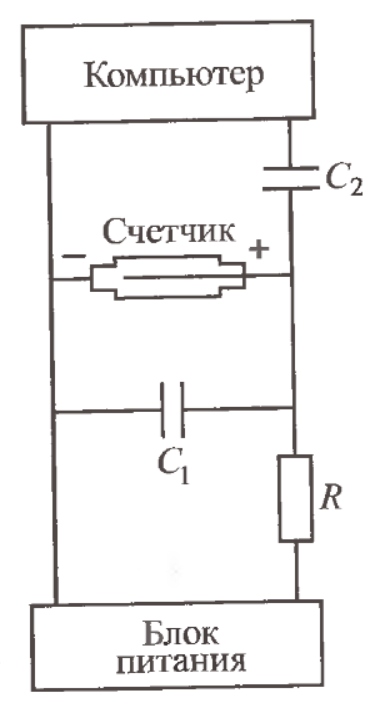
\includegraphics[width=0.175\textwidth]{счетчик}
\caption{Схема включения счетчика} \label{sch}
\end{wrapfigure}


Космические лучи обнаруживают с помощью ионизации, которую они производят, используя счетчик Гейгера-Мюллера. Схема его подключения приведена на рисунке \ref{sch}. Счетчик представляет собой наполненный гахом сосуд с двумя электродами. Частицы космических лчей ионизируют газ, выбивают электроны из стенок сосуда. Те, сталкиваясь с молекулами газа, выбивают из них электроны. Таким образом, получается лавина электронов, следовательно, через счетчик резко увеличивается ток. 

Погрешность измерения потока частиц с помощью счетчика Гейгера-Мюллера мала по сравнению с изменениями самого потока, то есть его флуктуациями.
\newpage
\section{Результаты измерений и обработка данных}

Результаты измерения числа частиц представлены в таблице \ref{20c}. Распределение числа срабатываний счетчика для 10 с и 40 с представлено в таблицах \ref{10c} и \ref{40c} соответсвенно.


\begin{table}
\caption{Число срабатываний счетчика за 20 с} \label{20c}
\begin{tabular}{|c|c|c|c|c|c|c|c|c|c|c|}
\hline 
№ опыта : & 1 & 2 & 3 & 4 & 5 & 6 & 7 & 8 & 9 & 10 \\ 
\hline 
0 : & 27 & 29 & 24 & 32 & 30 & 35 & 20 & 24 & 27 & 22 \\ 

10 : & 30 & 29 & 31 & 19 & 25 & 26 & 31 & 20 & 28 & 33 \\ 
 
20 : & 18 & 35 & 22 & 30 & 32 & 35 & 27 & 25 & 25 & 18 \\ 

30 : & 39 & 26 & 30 & 42 & 24 & 37 & 31 & 27 & 32 & 25 \\ 

40 : & 26 & 25 & 22 & 34 & 29 & 24 & 24 & 31 & 28 & 29 \\ 

50 : & 31 & 31 & 27 & 28 & 18 & 33 & 21 & 28 & 27 & 21 \\ 
 
60 : & 32 & 21 & 42 & 19 & 33 & 27 & 31 & 27 & 23 & 26 \\ 
 
70 : & 28 & 26 & 29 & 25 & 39 & 33 & 36 & 26 & 18 & 29 \\ 

80 : & 25 & 27 & 34 & 27 & 25 & 26 & 36 & 21 & 34 & 29 \\ 

90 : & 20 & 32 & 31 & 27 & 17 & 30 & 24 & 25 & 22 & 28 \\ 

100 : & 25 & 33 & 40 & 31 & 28 & 30 & 27 & 33 & 26 & 27 \\ 

110 : & 26 & 23 & 25 & 31 & 30 & 37 & 28 & 29 & 28 & 21 \\ 

120 : & 23 & 33 & 29 & 31 & 23 & 29 & 30 & 27 & 17 & 31 \\ 

130 : & 24 & 29 & 20 & 28 & 40 & 20 & 25 & 29 & 31 & 32 \\ 

140 : & 30 & 15 & 24 & 29 & 28 & 26 & 36 & 24 & 20 & 31 \\ 

150 : & 27 & 20 & 27 & 32 & 25 & 34 & 34 & 32 & 28 & 34 \\ 

160 : & 31 & 24 & 20 & 25 & 17 & 31 & 33 & 21 & 33 & 26 \\ 

170 : & 28 & 24 & 34 & 34 & 26 & 25 & 27 & 16 & 20 & 27 \\ 

180 : & 34 & 27 & 22 & 23 & 32 & 26 & 25 & 25 & 30 & 18 \\ 

190 : & 35 & 27 & 31 & 38 & 31 & 27 & 25 & 25 & 42 & 38 \\ 

\hline 
\end{tabular} 
\end{table}


\begin{table}
\caption{Данные для построения гистограммы распределения числа срабатываний счетчика за 10 с} \label{10c}
\begin{tabular}{|c|c|c|c|c|c|}
\hline 
Число импульсов $n_i$ & 4 & 5 & 6 & 7 & 8 \\ 
\hline 
Число случаев & 1 & 1 & 1 & 8 & 14 \\ 
\hline 
Доля случаев $w_n$ & 0.0025 & 0.0025 & 0.0025 & 0.002 & 0.035 \\ 
\hline 
\hline 
Число импульсов $n_i$ & 9 & 10 & 11 & 12 & 13 \\ 
\hline 
Число случаев & 23 & 28 & 43 & 30 & 35 \\ 
\hline 
Доля случаев $w_n$ & 0.0575 & 0.07 & 0.1075 & 0.075 & 0.0875 \\ 
\hline 
\hline 
Число импульсов $n_i$ & 14 & 15 & 16 & 17 & 18 \\ 
\hline 
Число случаев & 48 & 42 & 32 & 31 & 20 \\ 
\hline 
Доля случаев $w_n$ & 0.12 & 0.105 & 0.08 & 0.0775 & 0.05 \\ 
\hline 
\hline 
Число импульсов $n_i$ & 19 & 20 & 21 & 22 & 23 \\ 
\hline 
Число случаев & 11 & 13 & 7 & 7 & 1 \\ 
\hline 
Доля случаев $w_n$ & 0.0275 & 0.0325 & 0.0175 & 0.0175 & 0.0025 \\ 
\hline 
\hline 
Число импульсов $n_i$ & 24 & 25 & 26 & 27 & 28\\ 
\hline 
Число случаев & 0 & 1 & 2 & 0 & 1\\ 
\hline 
Доля случаев $w_n$ & 0 & 0.0025 & 0.005 & 0 & 0.0025\\ 
\hline 

\end{tabular} 
\end{table}

\begin{table}
\caption{Данные для построения гистограммы распределения числа срабатываний счетчика за 40 с} \label{40c}
\begin{tabular}{|c|c|c|c|c|c|c|c|}
\hline 
Число импульсов $n_i$ & 43 & 44 & 45 & 47 & 48 & 49 & 50\\ 
\hline 
Число случаев & 2 & 1 & 3 & 4 & 5 & 6 & 4 \\ 
\hline 
Доля случаев $w_n$ & 0.02 & 0.01 & 0.03 & 0.04 & 0.05 & 0.06 & 0.04 \\ 
\hline 
\hline 
Число импульсов $n_i$ & 51 & 52 & 53 & 54 & 55 & 56 & 57\\ 
\hline 
Число случаев & 7 & 6 & 6 & 5 & 3 & 5 & 5 \\ 
\hline 
Доля случаев $w_n$ & 0.07 & 0.06 & 0.06 & 0.05 & 0.03 & 0.05 & 0.05 \\ 
\hline 
\hline 
Число импульсов $n_i$ & 58 & 59 & 60 & 61 & 62 & 63 & 65\\ 
\hline 
Число случаев & 7 & 4 & 5 & 5 & 4 & 2 & 2 \\ 
\hline 
Доля случаев $w_n$ & 0.07 & 0.04 & 0.05 & 0.05 & 0.04 & 0.02 & 0.02 \\ 
\hline 
\hline
Число импульсов $n_i$ & 66 & 67 & 68 & 69 & 71 & 72 & 80\\ 
\hline 
Число случаев & 1 & 2 & 1 & 1 & 1 & 2 & 1 \\ 
\hline 
Доля случаев $w_n$ & 0.01 & 0.02 & 0.01 & 0.01 & 0.01& 0.02 & 0.01 \\ 
 
\hline 

\end{tabular} 
\end{table}
Представим результаты распределений в виде гистограммы, гистограмма распределения для $\tau=\text{40 c}$ обозначена синим цветом (рис. \ref{gist})

\begin{figure}[h!]
\begin{center}
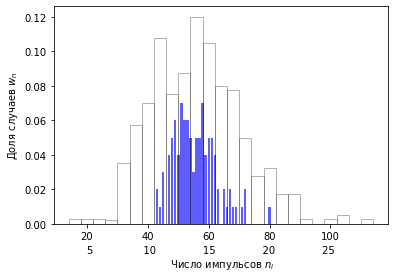
\includegraphics[width=0.9\textwidth]{gist}
\caption{Гистограммы для $\tau=\text{10 c}$ и $\tau=\text{40 c}$} \label{gist}
\end{center}

\end{figure}

Определим среднее число частиц за 10 и 40 с, $N_{10}=400$, $N_{40}=100$:
\[\overline{n_{10}}=\frac{1}{N_{10}}\sum_{i=1}^{N_{10}} {n_i}=\frac{5557}{400}=13.893\]
\[\overline{n_{40}}=\frac{1}{N_{40}}\sum_{i=1}^{N_{40}} {n_i}=\frac{5557}{100}=55.57\]
Найдем среднеквадратичную ошибку отдельного измерения за 10 и 40 с по формуле \ref{сигмаотд}:
\[\sigma_{\text{отд10}}=\sqrt{\frac{1}{N_{10}}\sum_{i=1}^{N_{10}}{(n_i-\overline{n_{10}})^2}}=3.78\]
\[\sigma_{\text{отд40}}=\sqrt{\frac{1}{N_{40}}\sum_{i=1}^{N_{40}}{(n_i-\overline{n_{40}})^2}}=7.001\]

Убедимся в справедливости формулы \ref{сигмаотдприб}:
\[3.78\thickapprox\sqrt{13.893}=3.73\]
\[7.001\thickapprox\sqrt{55.57}=7.45\]

Определим долю случаев, когда отклонения от среднего значения не превышают $\sigma_{\text{отд10}}$, $2\sigma_{\text{отд10}}$ и сравним с теоритическими значениями:
\begin{table}
\begin{tabular}{|c|c|c|c|}
\hline 
Ошибка & Число случаев & Доля случаев, \% & Теоретическая оценка \\ 
\hline 
$\pm \sigma_{\text{отд10}}=\pm3.78$& 261 & 65 & 68 \\ 

$\pm 2\sigma_{\text{отд10}}=\pm7.56$ & 385 & 96 & 95 \\ 
\hline 
\end{tabular}
\end{table}
 
Определим аналогичную долю случаев для $t=\text{40 c}$ и сравним с теоритическими значениями:
\begin{table}
\begin{tabular}{|c|c|c|c|}
\hline 
Ошибка & Число случаев & Доля случаев, \% & Теоретическая оценка \\ 
\hline 
$\pm \sigma_{\text{отд10}}=\pm7.001$& 72 & 72 & 68 \\ 

$\pm 2\sigma_{\text{отд10}}=\pm14.002$ & 96 & 96 & 95 \\ 
\hline 
\end{tabular} 
\end{table}


Найдем среднеквадратичное отклонение для средних значений по формуле \ref{сигманср}:

\[\sigma_{\overline{n_{10}}}=\frac{1}{N_{10}}\sqrt{\sum_{i=1}^{N_{10}}{(n_i-\overline{n_{10}})^2}}=\frac{\sigma_{\text{отд10}}}{\sqrt{N_{10}}}=0.19\]

\[\sigma_{\overline{n_{40}}}=\frac{1}{N_{40}}\sqrt{\sum_{i=1}^{N_{40}}{(n_i-\overline{n_{40}})^2}}=\frac{\sigma_{\text{отд40}}}{\sqrt{N_{40}}}=0.7\]

И получим окончательный результат для $n_{10}$ и $n_{40}$:
\[n_{10}=\overline{n_{10}}\pm\sigma_{\overline{n_{10}}}=13.893\pm0.19\]
\[n_{40}=\overline{n_{40}}\pm\sigma_{\overline{n_{40}}}=55.57\pm0.7\]
\section{Вывод}
Получены случайно изменяющиеся со временем данные об интенсивности потока космических частиц. Применены методы обработки данных для изучения статистических закономерностей при измерении интенсивности радиационного фона.
\end{document}